\documentclass[tikz,border=10pt]{standalone}
\usepackage{tikz}
\usepackage{adjustbox}
\usepackage{fontawesome5}
\usetikzlibrary{arrows.meta,positioning,fit,backgrounds,calc,shadows,shapes.geometric}

% Lavender & Legal RAG Color Palette
\definecolor{lavenderDark}{RGB}{15, 44, 89}
\definecolor{lavenderDeep}{RGB}{10, 28, 58}
\definecolor{lavenderMedium}{RGB}{29, 78, 158}
\definecolor{lavenderLight}{RGB}{240, 246, 255}
\definecolor{lavenderBorder}{RGB}{180, 205, 237}
\definecolor{lavenderAccent}{RGB}{2, 132, 199}
\definecolor{prismNavy}{RGB}{15, 44, 89}
\definecolor{prismBlue}{RGB}{29, 78, 158}
\definecolor{prismTeal}{RGB}{13, 148, 136}
\definecolor{prismMint}{RGB}{236, 253, 245}
\definecolor{prismGold}{RGB}{217, 119, 6}
\definecolor{prismDark}{RGB}{15, 23, 42}
\definecolor{prismLight}{RGB}{248, 250, 252}
\definecolor{cInput}{RGB}{241, 245, 249}
\definecolor{cStem}{RGB}{224, 242, 254}
\definecolor{cStage1}{RGB}{209, 250, 229}
\definecolor{cStage2}{RGB}{254, 243, 199}
\definecolor{cStage3}{RGB}{254, 226, 226}
\definecolor{cStage4}{RGB}{207, 250, 254}
\definecolor{cHead}{RGB}{219, 234, 254}
\definecolor{cOutput}{RGB}{255, 228, 230}

\begin{document}
\begin{tikzpicture}[
  >=Latex,
  stagebox/.style={
    draw=lavenderDark!85,
    rounded corners=7pt,
    minimum height=5.50cm,
    text width=2.65cm,
    align=center,
    inner sep=5pt,
    line width=1.1pt,
    fill=white,
    drop shadow={shadow xshift=1.5pt, shadow yshift=-1.8pt, opacity=0.16}
  },
  pipearrow/.style={
    ->,
    draw=lavenderDark,
    line width=1.8pt,
    arrows={-Latex[length=3.2mm, width=2.4mm]}
  }
]

  % Stage 1: PDF Ingestion
  \node[stagebox, fill=cInput!65] (ingest) {
    \vspace{3pt}
    {\fontsize{16}{18}\selectfont\textcolor{lavenderDark}{\faFilePdf}}\\[4pt]
    {\fontsize{10.0}{12.0}\selectfont\textbf{1. PDF Ingestion}}\\[2pt]
    {\fontsize{7.0}{8.2}\selectfont\textcolor{prismTeal}{\textbf{[Corpus Acquisition]}}}\\[5pt]
    \rule{2.3cm}{0.6pt}\\[6pt]
    \begin{minipage}{2.45cm}
      \fontsize{7.8}{9.6}\selectfont
      $\bullet$ Legal PDF corpus\\
      $\bullet$ User document upload\\
      $\bullet$ MIME validation\\
      $\bullet$ PyMuPDF (fitz) text\\
      $\bullet$ Page-numbered blocks\\
      $\bullet$ Payload guard $\le 50$\,MB
    \end{minipage}
    \vspace{4pt}
  };

  % Stage 2: Text Preprocessing & Chunking
  \node[stagebox, fill=cStage1!60, right=0.22cm of ingest] (preprocess) {
    \vspace{3pt}
    {\fontsize{16}{18}\selectfont\textcolor{prismTeal}{\faStream}}\\[4pt]
    {\fontsize{10.0}{12.0}\selectfont\textbf{2. Text Chunker}}\\[2pt]
    {\fontsize{7.0}{8.2}\selectfont\textcolor{prismTeal}{\textbf{[Token Overlap]}}}\\[5pt]
    \rule{2.3cm}{0.6pt}\\[6pt]
    \begin{minipage}{2.45cm}
      \fontsize{7.8}{9.6}\selectfont
      $\bullet$ Clean headers/footers\\
      $\bullet$ Whitespace normalization\\
      $\bullet$ Word chunking ($c=900$)\\
      $\bullet$ Overlap window ($o=150$)\\
      $\bullet$ Filter fragments $<40$w\\
      $\bullet$ Preserve source metadata
    \end{minipage}
    \vspace{4pt}
  };

  % Stage 3: Embedding Generation
  \node[stagebox, fill=cStem!60, draw=lavenderDark!95, line width=1.3pt, right=0.20cm of preprocess] (embed) {
    \vspace{3pt}
    {\fontsize{16}{18}\selectfont\textcolor{lavenderDark}{\faBrain}}\\[4pt]
    {\fontsize{10.0}{12.0}\selectfont\textbf{3. SBERT Embed}}\\[2pt]
    {\fontsize{7.0}{8.2}\selectfont\textcolor{lavenderDark}{\textbf{[Semantic Vectors]}}}\\[5pt]
    \rule{2.3cm}{0.6pt}\\[6pt]
    \begin{minipage}{2.45cm}
      \fontsize{7.8}{9.6}\selectfont
      $\bullet$ Sentence-Transformers\\
      $\bullet$ \texttt{all-MiniLM-L6-v2}\\
      $\bullet$ 384-dimensional dense\\
      $\bullet$ Unit L2 normalization\\
      $\bullet$ Fast CPU inference\\
      $\bullet$ Semantic similarity map
    \end{minipage}
    \vspace{4pt}
  };

  % Stage 4: Pinecone Indexing
  \node[stagebox, fill=cStage4!60, right=0.22cm of embed] (index) {
    \vspace{3pt}
    {\fontsize{16}{18}\selectfont\textcolor{lavenderDark}{\faDatabase}}\\[4pt]
    {\fontsize{10.0}{12.0}\selectfont\textbf{4. Vector Index}}\\[2pt]
    {\fontsize{7.0}{8.2}\selectfont\textcolor{lavenderDark}{\textbf{[HNSW Indexing]}}}\\[5pt]
    \rule{2.3cm}{0.6pt}\\[6pt]
    \begin{minipage}{2.45cm}
      \fontsize{7.8}{9.6}\selectfont
      $\bullet$ Pinecone cloud index\\
      $\bullet$ Cosine metric\\
      $\bullet$ Batch upsert (100 vec)\\
      $\bullet$ Document metadata tags\\
      $\bullet$ Sub-100ms ANN lookup\\
      $\bullet$ 1M capacity tier
    \end{minipage}
    \vspace{4pt}
  };

  % Stage 5: Retrieval & Gemini Generation
  \node[stagebox, fill=cStage2!65, draw=prismGold!95!black, line width=1.2pt, right=0.22cm of index] (generate) {
    \vspace{3pt}
    {\fontsize{16}{18}\selectfont\textcolor{prismGold!95!black}{\faComments}}\\[4pt]
    {\fontsize{10.0}{12.0}\selectfont\textbf{5. LLM Synthesis}}\\[2pt]
    {\fontsize{7.0}{8.2}\selectfont\textcolor{prismGold!95!black}{\textbf{[Grounded QA]}}}\\[5pt]
    \rule{2.3cm}{0.6pt}\\[6pt]
    \begin{minipage}{2.45cm}
      \fontsize{7.8}{9.6}\selectfont
      $\bullet$ Query top-$k$ retrieval\\
      $\bullet$ Google Gemini 2.5 Flash\\
      $\bullet$ Context prompt assembly\\
      $\bullet$ Statutory section cites\\
      $\bullet$ Malayalam translation\\
      $\bullet$ Zero hallucination guard
    \end{minipage}
    \vspace{4pt}
  };

  % Pipeline Flow Arrows
  \draw[pipearrow] (ingest) -- (preprocess);
  \draw[pipearrow] (preprocess) -- (embed);
  \draw[pipearrow] (embed) -- (index);
  \draw[pipearrow] (index) -- (generate);

\end{tikzpicture}
\end{document}
